%!TEX root = main.tex
\section{Details in Section~\ref{sec:symbolic}: Symbolic extensions}\label{app-sym}

In this section, we add the details of Section~\ref{sec:symbolic}, especially the complexity analysis of the decision procedure.

\subsection{Some definitions, notations, and basic facts}

We first make it explicit the definition of symbolic automata. 

\begin{definition}[Symbolic automata]\label{def-2sa}
    A (nondeterministic two-way)  symbolic automata (\SSA) is a tuple $\Aut = (\EndLeft, \EndRight, \controls, q_0, \finals, \transrel)$, where  
\begin{itemize}
%\item $\Upsilon=(\signature, \structure, \Psi)$ is a decidable Boolean algebra, where $\signature = (\functions, \predicates)$ and $\structure = (\data, \interpretation)$,
%
\item $\EndLeft$, $\EndRight$, $\controls$, $q_0$, $\finals$ are defined precisely as in \FFA{}s, 
%
\item $\transrel$ is a finite set of transitions of one of the following forms,
\begin{itemize}
\item     symbolic transitions $(q, \psi(x), dir, q') \in \controls \times \Psi \times \{\Left, \Stay, \Right\} \times \controls$, where $q, q'$ are the source and target state, $dir$ is the direction, and $\psi(x)$ is the guard of the transition, 
%
\item     non-symbolic transitions $(q, \EndLeft, dir, q')$ with $dir \in \{\Right, \Stay\}$, or $(q, \EndRight, dir', q')$ with $dir' \in \{\Left,\Stay\}$. 
\end{itemize}
\end{itemize}
A \SSA{} is an \SA{} if there are no transitions with the direction ``$\Left$". 
%for each $(q, \psi(x), dir, q')$, we have $dir \in \{\Stay, \Right\}$, moreover, the transitions of the form $(q, \EndRight, \Left, q')$ are removed.
\end{definition}

%%%====================semantics removed=============================
%%%====================semantics removed=============================
\hide{
\paragraph{Semantics of \SSA{} $\Aut = (\Upsilon, \EndLeft, \EndRight, \controls, q_0, \finals, \transrel)$.}
A transition $\tau=(q_1,\psi(x), dir, q_2) \in \transrel$ in the \SSA{}  can be concretised
into a potentially infinite set of \emph{concrete} transitions $\|\tau\| \subseteq Q \times \data \times \{\Left, \Stay, \Right\} \times Q$, where $(q_1, d, dir, q_2)  \in \|\tau\|$ iff $d \in \|\psi\|$.
Intuitively, suppose $\Aut$ is at the state $q_1$ and reading the input data value $d \in \data$.
If there is a transition $(q_1, \psi(x), dir, q_2) \in \transrel$ such that $d \in \|\psi\|$, then $\Aut$ can move its reading head according to $dir$, and change the state from $q_1$ to $q_2$.

%$\Aut$ is interpreted on \emph{data strings}, namely, elements of $\data^*$.
Given a data string $w = d_1, \dots, d_n$, a \emph{run} of $\Aut$ on $w$
is a sequence of tuples $(q_0, i_0), \ldots, (q_m, i_m) \in \controls \times [0, n+1]$ 
such that
%let $d_0 = \EndLeft$ and $d_{n+1} = \EndRight$, %. The following conditions, then, have to be satisfied:
\begin{itemize}
    \item $i_0 = 0$, and
    \item for every $j \in [m-1]$, one of the following holds,
    \begin{itemize}
  	\item $0 < i_j < n+1$,  and $\tau=(q_j, \psi(x), dir, q_{j+1}) \in \transrel$ for some $\psi(x) \in \Psi$ and $dir \in \{\Left, \Stay, \Right\}$, such that $(q_j, d_{i_j}, dir, q_{j+1}) \in \|\tau\|$, and $i_{j+1} = i_j + dir$,
	%
	\item $i_j = 0$, $(q_j, \EndLeft, dir, q_{j+1}) \in \transrel$, and $i_{j+1} = i_j + dir$,
	%
	\item $i_j = n+1$, $(q_j, \EndRight, dir, q_{j+1}) \in \transrel$, and $i_{j+1} = i_j + dir$.
  \end{itemize}
\end{itemize}
The run is said to be \defn{accepting} if $i_m = n+1$ and $q_m \in \finals$.
A data string $w$ is accepted by $\Aut$ if there is an accepting run of
$\Aut$ on $w$. We use $\Lang(\Aut)$ to denote the data language recognised by $\Aut$, that is,  the set of data strings accepted by $\Aut$.
%
For simplicity, we usually omit $\EndLeft$, and $\EndRight$ from the definition of \SSA{}s. 
}
%%%====================semantics removed=============================

\paragraph{Size measures}
We first assume that given a formula $\psi \in \Psi$ of size $m$ in $\Upsilon$, $\issat(\psi)$ can be decided in $\bigO(\beta(m))$ space for some monotone function $\beta$ such that $\beta(m) \ge \log m$. We also assume that the formulae and terms in $\Upsilon$ are encoded in a proper way, e.g. encoded in binary,  and let $|\psi|$  and $|t|$ to denote the size (i.e. number of symbols) of $\psi$ and $t$ with respect to this encoding.

Let $\Transducer$ be a \SSPT{}. We define $|\Transducer|_s$ and $|\Transducer|_d$, the \emph{structural and data size} of $\Transducer$, by taking the guards and outputs of transitions (from the background theory $\Upsilon$) into consideration. Specifically, $|\Transducer|_s$ is defined as the product of the number of transitions and the maximum length of sequences of $\signature$-terms in  transitions of $\Transducer$; 
$|\Transducer|_d$ is defined as the maximum size of symbolic transitions of $\Transducer$, where the size of a symbolic transition $(q, \psi(x), dir, q', \vec{t}(x))$ with $\vec{t}=t_1 \ldots t_r$ is defined as $|\psi| + |t_1| + \ldots + |t_r|$.

The size measures of \SSA{}s are defined similarly, specifically, $|\Aut|_s$  is  defined as the number of transitions of $\Aut$, and $|\Aut|_d$ is defined as the maximum size of symbolic transitions of $\Aut$, where the size of a symbolic transition $(q, \psi(x), dir, q')$ is defined as $|\psi|$. 

Then we state and prove some basic facts about \SSA{}s.
\begin{proposition}\label{prop-2nsa}
Assume a \SSA{}  $\Aut$. Then
\begin{itemize}
\item $\Aut$ can be  transformed into an equivalent \SA{} $\Aut'$ in time $|\Aut'|_s \cdot |\Aut'|_d$, where $|\Aut'|_s = 2^{\bigO\left(|\Aut|_s \log |\Aut|_s\right)}$ and $|\Aut'|_d = \bigO(|\Aut|_s |\Aut|_d)$;
%$|\Aut'| = 2^{O (|\Aut| \log |\Aut| )}$.
%
%
%\item SAs are under the intersection operator\footnote{As a matter of fact, SAs are closed under all Boolean operations. Since we only use the intersection in this paper, we restrict our attention to the intersection.}. \zhilin{complexity}
%
\item the nonemptiness of $\Aut$ can be decided in nondeterministic $\bigO( (\log |\Aut|_s) + \beta(|\Aut|_d))$ space.
\end{itemize}
\end{proposition}


\begin{proof}
The proof the second result is obtained by guessing a path in $\Aut$ and was shown in \cite{NG01,DV14}.

Next, we prove the first result.

Let $\Aut = (\Upsilon, \EndLeft, \EndRight, \controls, q_0, \finals, \transrel)$ be a \SSA. We show how to construct an equivalent \SA{} $\Aut' =  (\Upsilon, \controls', q'_0, \finals', \transrel')$.
W.l.o.g., we assume that for each transition $(q, \psi, dir, q') \in \transrel$, we have $dir \in \{\Left,\Right\}$. Every \SSA{} can be turned into one \SSA{} satisfying the assumption as follows: Replace each transition $(q, \psi, \Stay, q') \in \transrel$ with three new transitions $(q, \psi, \Right, q'')$, $(q'', \ltrue, \Left, q')$, and $(q'', \EndRight, \Left, q')$, where $q''$ is a fresh state.

The proof is an adaptation of the construction of \FA{} from \FFA{} based on the notion of crossing sequences (cf., e.g., \cite{HU79}). Since \SSA{}s replace the letters in \FFA{}s with unary predicates, the main technical challenge here is to deal with these predicates (i.e., guards).

We first use an example to illustrate the idea of crossing sequences: Suppose $w = \EndLeft d_1 d_2 d_3 d_4 d_5\EndRight$, and an accepting run of $\Aut$ on $w$ uses the following sequence of transitions 
\[
\begin{array}{l}
(q_0, \EndLeft, \Right, q_1), (q_1, \psi_1, \Right, q_1), (q_1, \psi_2, \Left, q_2), (q_2, \psi_3, \Right, q_0), (q_0, \psi_4, \Right, q_1), \\
(q_1, \psi_1, \Right, q_1), (q_1, \psi_1, \Right, q_1), (q_1, \psi_2, \Left, q_2), (q_2, \psi_3, \Right, q_0), (q_0, \psi_4, \Right, q_1),
\end{array}
\] 
with $q_1 \in \finals$.
(The run is illustrated in Figure~\ref{fig-2sa-sa}.) A \emph{crossing sequence} of the run is a sequence of states on the boundary of two tape cells, e.g. the sequence $q_1, q_2, q_0$ on the boundary of $d_1$ and $d_2$. Note that for technical convenience, the states of the run are put in a way that, whenever a left-transition $(q, \psi, \Left, q')$ is taken, $q'$ is put just below $q$, thus in the \emph{same} crossing sequence as $q$ rather than the cross sequence of th position on the left. Therefore, 
\emph{the target state of each left-transition is put in the position right-adjacent to the actual position of the reading head}.
For instance, in Figure~\ref{fig-2sa-sa}, when the transition $(q_1, \psi_2, \Left, q_2)$ is taken, $q_2$ is put just below $q_1$. Different from the crossing sequences for 2FAs, in Figure~\ref{fig-2sa-sa}, naturally we also include the guards of the transitions. 

\begin{figure}[htbp]
\begin{center}
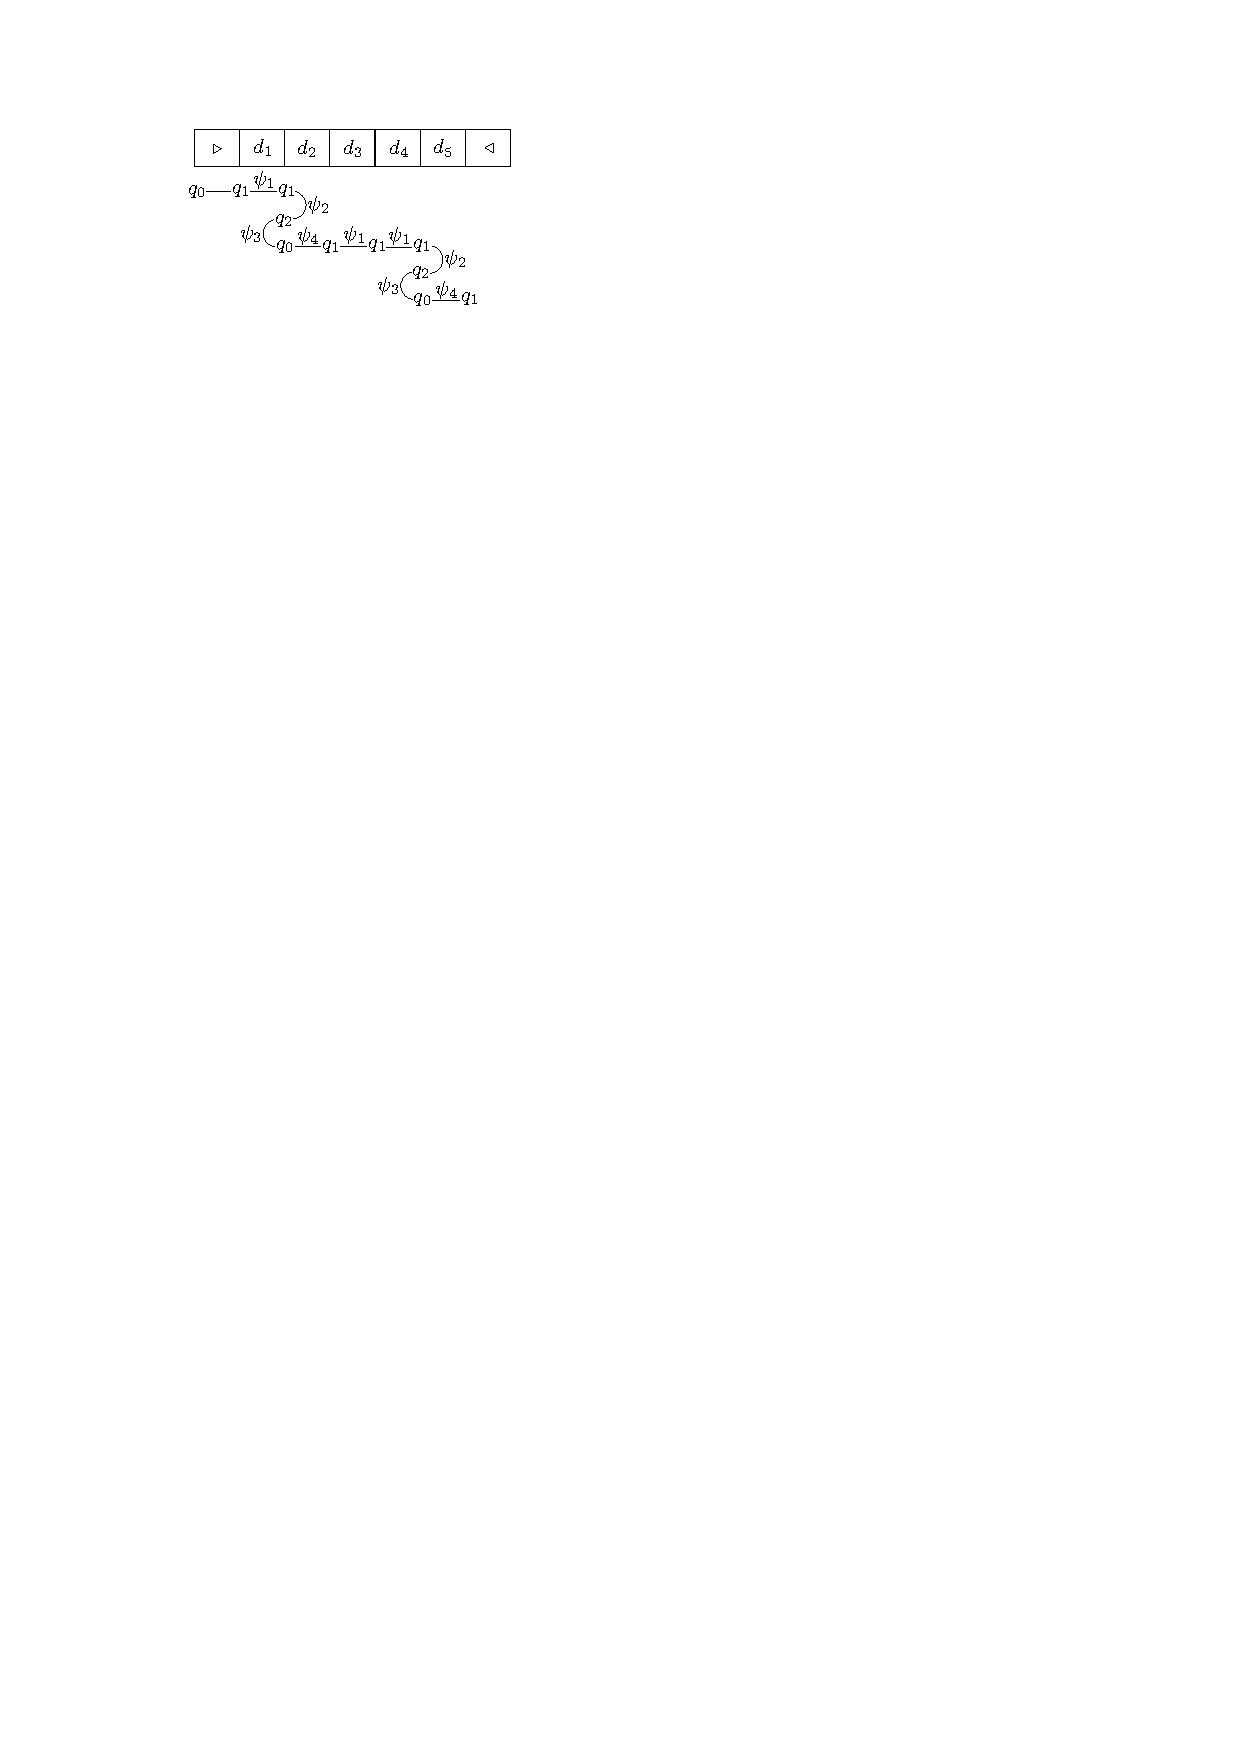
\includegraphics{2sa-sa-exmp.pdf}
\end{center}
\caption{Accepting runs of $\Aut$: An example}\label{fig-2sa-sa}
\end{figure}

In order to deal with the guards in the transitions, we adapt the crossing sequences of the \SSA{} $\Aut$  as follows: a crossing sequence of $\Aut$ is a sequence of \emph{transitions} of odd lengths such that  the source states of the transitions in the even and odd  positions respectively are mutually distinct. Let $S_\transrel$ denote the set of such sequences of transitions. 
%Notice that, in general, any $\rho\in S_\transrel$  is of the form that $\rho = \tau_1, \ldots, \tau_{2n+1}$ for some $n$ such that for each $i \in [n+1]$, $\tau_{2i-1} = (p_{2i-1}, \EndRight, \Left, q_{2i-1})$, and for each $i \in [n]$, $\tau_{2i} = (p_{2i}, \psi_{2i}, dir_{2i}, q_{2i})$.


\newcommand\lmatch{\mathsf{LeftMatch}}
\newcommand\rmatch{\mathsf{RightMatch}}

In order to construct the set of transitions of $\Aut'$, we shall define two \emph{partial} functions $\lmatch(\rho_1, \rho_2)$ and $\rmatch(\rho_1, \rho_2)$ for $\rho_1, \rho_2 \in S_\transrel$. 
The intention of $\lmatch(\rho_1, \rho_2)$ and $\lmatch(\rho_1, \rho_2)$ is explained as follows.
\begin{itemize}
\item The intention of $\lmatch(\rho_1, \rho_2)$: $\rho_1$ and $\rho_2$ are the crossing sequences to the left resp. right of some position $i$ holding a data value $d$. Initially, we reach the source state of the first transition of $\rho_2$ by a \emph{left-transition} (thus after this transition, the reading head is in the position $i$\footnote{Recall that the target state of each left-transition is put in the position right-adjacent to the actual position of the reading head.}).
%
\item The intention of $\rmatch(\rho_1, \rho_2)$:  $\rho_1$ and $\rho_2$ are the crossing sequences to the left resp. right of some position $i$ holding a data value $d$. Initially, we reach the source state of the first transition of $\rho_1$ %, say $p_1$, 
by a \emph{right-transition} (thus after this transition, the reading head is in the position $i$).
\end{itemize}
%
Formally, the domain of $\lmatch$ (resp. $\rmatch$) is defined inductively as follows, where in each case below, the return value is also specified. Let $\rho_1, \rho_2 \in S_\transrel$. Then $\lmatch(\rho_1, \rho_2)$ is defined iff one of the following constraints holds.
\begin{itemize}
\item Case $\rho_1 = \varepsilon$, $\rho_2 = \varepsilon$: $\lmatch(\rho_1, \rho_2) = \ltrue$.
%
\item Case $\rho_1 =  \tau_{1,1}, \ldots, \tau_{1,k}$ with $k \ge 1$, $\rho_2 = \tau_{2,1}, \ldots, \tau_{2,l}$ with $l \ge 1$, $\tau_{2,1} = (q_1, \psi_{2,1}, \Left, p_1)$, $p_1$ is the source state of $\tau_{1,1}$, and $\rmatch(\rho'_1, \rho'_2)$ is defined:  
$$\lmatch(\rho_1, \rho_2) = \psi_{2,1} \wedge \rmatch(\rho'_1, \rho'_2),$$ 
where $\rho'_1 = \tau_{1,2}, \ldots, \tau_{1,k}$ and $\rho'_2 = \tau_{2,2}, \ldots, \tau_{2,l}$.
%
\item Case $\rho_1 =  \tau_{1,1}, \ldots, \tau_{1,k}$ with $k \ge 1$, $\rho_2 = \tau_{2,1}, \ldots, \tau_{2,l}$ with $l \ge 1$, $\tau_{2,1} = (q_1, \psi_{2,1}, \Right, q_2)$, $q_2$ is the source state of $\tau_{2,2}$, and $\lmatch(\rho_1, \rho'_2)$ is defined:  
$$\lmatch(\rho_1, \rho_2) = \psi_{2,1} \wedge \lmatch(\rho_1, \rho'_2),$$ 
where $\rho'_2 = \tau_{2,3}, \ldots, \tau_{2,l}$.
%
\end{itemize} 
%
Symmetrically, $\rmatch(\rho_1, \rho_2)$ is defined iff one of the following constraints holds.
\begin{itemize}
\item Case $\rho_1 = \varepsilon$, $\rho_2 = \varepsilon$: $\rmatch(\rho_1, \rho_2) = \ltrue$.

\item Case $\rho_1 =  \tau_{1,1}, \ldots, \tau_{1,k}$ with $k \ge 1$, $\rho_2 = \tau_{2,1}, \ldots, \tau_{2,l}$ with $l \ge 1$, $\tau_{1,1} = (p_1, \psi_{1,1}, \Right, q_1)$, $q_1$ is the source state of $\tau_{2,1}$, and $\lmatch(\rho'_{1}, \rho'_2)$ is defined:  
$$\rmatch(\rho_1, \rho_2) =\psi_{1,1} \wedge \lmatch(\rho'_{1}, \rho'_2),$$ 
where $\rho'_1 = \tau_{1, 2},\ldots, \tau_{1,k}$, and $\rho'_2 = \tau_{2,2}, \ldots, \tau_{2,l}$.
%
\item Case $\rho_1 =  \tau_{1,1}, \ldots, \tau_{1,k}$ with $k \ge 1$, $\rho_2 = \tau_{2,1}, \ldots, \tau_{2,l}$ with $l \ge 1$, $\tau_{1,1} = (p_1, \psi_{1,1}, \Left, p_2)$, $p_2$ is the source state of $\tau_{1,2}$, and $\rmatch(\rho'_1, \rho_2)$ is defined:  
$$\rmatch(\rho_1, \rho_2) = \psi_{1,1} \wedge \rmatch(\rho'_1, \rho_2),$$ 
where $\rho'_1 = \tau_{1,3}, \ldots, \tau_{1,k}$.
%
\end{itemize}
%
We are ready to construct the \SA{} $\Aut' =  (\Upsilon, \controls', q'_0, \finals', \transrel')$, where
\begin{itemize}
\item $\controls' = S_\transrel \cup \{q'_0\}$, where $q'_0$ is a fresh state,
%
\item $\finals'$ comprises the set of elements $\rho \in S_\transrel$ as follows: suppose $\rho = \tau_1, \ldots, \tau_{2n+1}$, where for each $i \in [n+1]$, $\tau_{2i-1} = (p_{2i-1}, \EndRight, \Left, q_{2i-1})$, and for each $i \in [n]$, $\tau_{2i} = (p_{2i}, \psi_{2i}, dir_{2i}, q_{2i})$, then $\rho$ must satisfy that $q_{2n+1} \in F$ and $q_{2i-1} = p_{2i}$ for each $i \in [n]$,  
%
\item $\transrel'$ comprises the following transitions: 
%
\begin{itemize}
%
\item $(\rho, \rmatch(\rho, \rho'), \rho') \in \transrel'$ for all $\rho, \rho' \in S_\transrel$ such that $\rmatch(\rho, \rho')$ is defined;
%
\item  
%the transitions out of $q'_0$ are defined as follows:
%
$(q'_0, \rmatch(\rho, \rho'), \rho') \in \transrel'$ for all $\rho \in I'$ and $\rho' \in S_\transrel$ such that $\rmatch(\rho, \rho')$ is defined, where 
$I'$ comprises $\rho'' \in S_\transrel$ satisfying the following constraints: $\rho'' = \tau_1, \ldots, \tau_{2n+1}$,  for each $i \in [n+1]$, $\tau_{2i-1} = (p_{2i-1}, \psi_{2i-1}, dir_{2i-1}, q_{2i-1})$, for each $i \in [n]$, $\tau_{2i} = (p_{2i}, \EndLeft, \Right, q_{2i})$. In addition, $(q_0, \EndLeft, \Right, p_1) \in \transrel$, and for each $i \in [n]$, $q_{2i} = p_{2i+1}$. 
\end{itemize}
%
\end{itemize}

Since $S_\transrel$ contains at most $(|\Aut|_s)^{2 |\controls|-1} \le (|\Aut|_s)^{2 |\Aut|_s}$ elements, we conclude that 
$$
\begin{array}{l c l}
|\Aut'|_s \le ((|\Aut|_s)^{2|\Aut|_s})^2  & = & (|\Aut|_s)^{4|\Aut|_s} 
 \approx    2^{\bigO\left(|\Aut|_s \log |\Aut|_s\right)}
\end{array}
$$ 
and 
$$
\begin{array}{l c l}
|\Aut'|_d \le 2(2|\controls|-1) |\Aut|_d & \le & 4 |\Aut|_s |\Aut|_d 
\approx   \bigO( |\Aut|_s |\Aut|_d).
\end{array}
$$
\end{proof}



%%%====================================================================
%%%====================================================================

\subsection{The details of the generic decision procedure}


Similar to recognisable relations, we also represent a  $\arity$-ary symbolic recognisable relation as a collection of tuples $(\Aut_1, \ldots, \Aut_\arity)$, where each atom $\Aut_i$ is a conjunctive representation of \SA{}, namely, of the form $((\controls, \transrel), \conacc)$ with $\conacc \subseteq \controls \times \controls$. We will use a conjunctive \SA{} to mean a conjunctive representation of the \SA{}. For a conjunctive \SA{} $\cC= ((\controls, \transrel), \conacc)$, two size measures $|\cC|_s$ and $|\cC|_d$ are defined similarly to \SA{}s. Moreover, the structural (resp. data) size of a representation of a symbolic recognisable relation is defined as the maximum structural (resp. data) size of the atoms.


The \prerec{} assumption in Section~\ref{sec:algo} is replaced by $\mathbb{S}$\prerec{} assumption presented below.
\begin{quote}
{\bf The $\mathbb{S}$\prerec{} assumption}. For each data string function $f$ in $S$ and each conjunctive \SA{} $\Aut$,  $f^{-1}(\Aut)$ is a symbolic recognisable relation. Furthermore, 
a representation of $f^{-1}(\Aut)$, whose structural size (resp. data size) is bounded by  $\ell_s(|f|_s, |\Aut|_s)$ (resp. $\ell_d(|f|_s,  |f|_d, |\Aut|_s, |\Aut|_d)$) for some monotone functions $\ell_s$ and $\ell_d$, can be computed effectively. We also assume that each disjunct of the representation of $f^{-1}(\Aut)$ can be enumerated in $\ell_s(|f|_s, |\Aut|_s) \cdot \ell_d(|f|_s,  |f|_d, |\Aut|_s,  |\Aut|_d)$ space.
%
\end{quote} 
%
Here $|f|_s$ and $|f|_d$ are the structural and data sizes of a representation of $f$ respectively; the concrete definitions depend on the form of $f$, which will be given when the generic decision procedure is instantiated later. Furthermore, we define the size of $f$ (resp. $\Aut$), denoted by $|f|$ (resp. $|\Aut|$), as $|f|_s \cdot |f|_d$ (resp. $|\Aut|_s \cdot |\Aut|_d$).

Let $S$ be a symbolic execution of programs with data strings.  We use $|S|$ to denote the sum of $|f|$ and $|\Aut|$ for data string functions $f$ and \SA{}s $\Aut$ occurring in $S$.  
For a refined complexity analysis, we also define $\rcdep(S)$, $\rcdim(S)$, and $\rcasrt(S)$ similarly to the string setting. Moreover, we use $\rcphi_s(S)$ (resp. $\rcphi_d(S)$) to denote the maximum of $|f|_s$ (resp. $|f|_d$) for data string functions $f$ occurring in the assignments of $S$, and $\rcpsi_s(S)$ (resp. $\rcpsi_d(S)$) to denote the maximum of $|\Aut|_s$ (resp. $|\Aut|_d$) for \SA{}s $\Aut$ occurring in $S$.


%Similarly, we can define $\numtrans(\psi)$ and $\sizetrans(\psi)$.


%We can adapt the definition of $\numtrans$ and $\sizetrans$ to the conjunctive representations of SA easily. We will use conjunctive SA to mean a conjunctive representation of the SA.

For a binary function $g(k, l)$, $h(i, j, k, l)$, and $n \in \Nat \backslash \{0\}$, we define $g^{\langle n \rangle}(k, l)$ and $h^{\langle n \rangle}_g(i, j, k, l)$ as follows: $g^{\langle 1 \rangle}( k, l) = g(k, l)$, $h^{\langle 1 \rangle}_g(i, j, k, l) = h(i, j, k, l)$, and 
$$g^{\langle n+1 \rangle}( k, l) = g(k, g^{\langle n \rangle}( k, l)), \ h^{\langle n+1 \rangle}_g (i, j, k, l) = h(i, j, g^{\langle n \rangle}(k, l), h^{\langle n \rangle}(i, j, k, l)).$$


\begin{theorem}\label{thm-generic-dec-symbolic}
	Given a symbolic execution  $S$ of programs with data strings satisfying the $\mathbb{S}$\prerec{} assumption, the path feasibility problem of $S$ can be decided in \emph{nondeterministic} $M+ \beta(M)$ space, where  
	\[
	\begin{array}{l c l}
%		M & = & |\vars(S)| \cdot (\rcdim(S)+1)^{\rcdep(S)}  \rcsreg(S) \cdot  (\ell_s^{\langle \rcdep(S) \rangle}(\rcphi_s(S), \rcpsi_s(S)))^{r}\ \cdot \\
		M & = & (\rcdim(S)+1)^{\rcdep(S)}  \rcasrt(S) \cdot  (\ell_s^{\langle \rcdep(S) \rangle}(\rcphi_s(S), \rcpsi_s(S)))^{c}\ \cdot \\
		& &  \hspace{1cm} (\ell_d)^{\langle  \rcdep(S) \rangle}_{\ell_s}(\rcphi_s(S),\rcphi_d(S),  \rcpsi_s(S), \rcpsi_d(S))
\end{array}
	\]
for some constant $c > 0$. 
\end{theorem}



%%%=============================================================
\hide{
\begin{theorem}\label{thm-generic-dec-symbolic}
Let $\transet$ be a class of symbolic parametric transducers. Suppose that %$\transet$ satisfies that 
for each $\Transducer \in \transet$ and conjunctive \SA{} $\Aut$, $\Pre_\Transducer(\Aut)$ is a symbolic recognisable relation and a representation of which can be computed effectively, 
such that for every atom $\Aut'$ therein, 
$\numtrans(\Aut') = O(g(\numtrans(\Transducer),  \numtrans(\Aut)))$ and 
$\sizetrans(\Aut') = O(h(\numtrans(\Transducer), \sizetrans(\Transducer), \numtrans(\Aut), \sizetrans(\Aut)))$, for two monotone functions $g$ and $h$.
Then the path feasibility of a $\straightlinesym[\transet]$ formula $\varphi \wedge \psi$ can be decided in nondeterministic space
$$
O\left(
\begin{array}{l}
(\rcdim(\varphi)+2)^{\rcdep(\varphi)}|\psi| \cdot (\numtrans'')^2 \log \numtrans'' + \\
f((\rcdim(\varphi)+2)^{\rcdep(\varphi)} (\numtrans'')^2 \sizetrans'')  
\end{array}
\right),
$$ 
where $\numtrans'' = g^{\langle \rcdep(\varphi) \rangle}(\numtrans(\varphi), \numtrans(\psi))$ and 
$$\sizetrans'' = h^{\langle \rcdep(\varphi) \rangle}_g(\numtrans(\Transducer), \sizetrans(\Transducer), \numtrans(\Aut), \sizetrans(\Aut)).$$
\end{theorem}
}
%%%=============================================================


\begin{proof}

For each $i$, let $N_{i,s}$ (resp. $N_{i, d}$) be the maximum structural size (resp. data size) of the conjunctive \SA{}s in $\bigcup \limits_{x \in \vars(S)} \cE_i(x)$. From the $\mathbb{S}$\prerec{} assumption and the fact that each string function $f$ satisfies  $|f|_s \le \rcphi_s(S)$ and $|f|_d \le \rcphi_d(S)$, we have 
%
$$N_{i-1, s} \le \ell_s(|f|_s, N_{i, s}) \le \ell_s(\rcphi_s(S), N_{i,s})$$ 
%
and
%
$$N_{i-1, d} \le \ell_d(|f|_s, |f|_d, N_{i, c}, N_{i,d}) \le \ell_d(\rcphi_s(S), \rcphi_d(S), N_{i, s}, N_{i,d}).$$ 

Because each conjunctive \SA{} in $\cE_{\rcdep(S)}(x)$ satisfies that its control and data size are bounded by $\rcpsi_c(S)$ and $\rcpsi_d(S)$ respectively, 
we have that each conjunctive \SA{} in $\cE(x)$ satisfies that its control and data size are bounded by $\ell_s^{\langle \rcdep(S) \rangle}(\rcphi_s(S), \rcpsi_s(S))$ and 
%
\[ (\ell_d)^{\langle  \rcdep(S) \rangle}_{\ell_s}(\rcphi_s(S), \rcphi_d(S), \rcpsi_s(S), \rcpsi_d(S)).\]
% h(i, j, g^{\langle n \rangle}(k, l), h^{\langle n \rangle}(i, j, k, l))
% 
Therefore, the size of each conjunctive \SA{} in $\cE(x)$ is bounded by 
{
\small
$$\ell_s^{\langle  \rcdep(S) \rangle}(\rcphi_s(S), \rcpsi_s(S)) \cdot (\ell_d)^{\langle \rcdep(S) \rangle}_{\ell_s}(\rcphi_s(S),  \rcphi_d(S), \rcpsi_s(S), \rcpsi_d(S)).$$
}
Furthermore, according to the $\mathbb{S}$\prerec{} assumption, the construction of these conjunctive \SA{}s can be done in nondeterministic space bounded by 
%
{
\small
$$\ell_s^{\langle  \rcdep(S) \rangle}(\rcphi_s(S), \rcpsi_s(S)) \cdot (\ell_d)^{\langle \rcdep(S) \rangle}_{\ell_s}(\rcphi_s(S),  \rcphi_d(S), \rcpsi_s(S), \rcpsi_d(S)) $$
}
as well.
%


For each $i$, let $M_i$ be the maximum number of elements in $\cE_i(x)$ for $x  \in \vars(S)$.
Then we have $M_{i-1} \le (\rcdim(S)+1)M_i $. Because for each $x \in \vars(S)$, $\cE_{\rcdep(S)}(x)$ contains at most $\rcasrt(S)$ elements, we have that for each $x \in \vars(S)$, $\cE(x)$ contains at most $(\rcdim(S)+1)^{\rcdep(S)}\rcasrt(S)$ elements. 

Therefore, for each $x \in \vars(S)$, the conjunctive product \SA{} $\Aut_x=((\controls_x, \transrel_x), \conacc_x)$ of these conjunctive \SA{}s  in $\cE(x)$ has a structural size bounded by 
%
$$(\ell^{\langle \rcdep(S) \rangle}_s(\rcphi_s(S), \rcpsi_s(S)))^{(\rcdim(S)+1)^{\rcdep(S)} \rcasrt(S)},$$
%
and data size bounded by
%
\[ (\rcdim(S)+1)^{\rcdep(S)} \rcasrt(S) (\ell_d)^{\langle  \rcdep(S) \rangle}_{\ell_s}(\rcphi_s(S),\rcphi_d(S),  \rcpsi_s(S), \rcpsi_d(S)) \]
%
and $|\conacc_x| \le (\ell_s^{\langle \rcdep(S) \rangle}(\rcphi_s(S), \rcpsi_s(S)))^2$. 
It follows that the structural and data size of the (standard) \SA{} corresponding to $\Aut_x$ are  bounded by 
%
$$(\ell^{\langle \rcdep(S) \rangle}_s(\rcphi_s(S), \rcpsi_s(S)))^{(\rcdim(S)+1)^{\rcdep(S)} \rcasrt(S) \left(\ell_s^{\langle \rcdep(S) \rangle}(\rcphi_s(S), \rcpsi_s(S))\right)^2}$$
%
and
$$
\begin{array}{l}
\left(\ell_s^{\langle \rcdep(S) \rangle}(\rcphi_s(S), \rcpsi_s(S))\right)^2 (\rcdim(S)+1)^{\rcdep(S)} \rcasrt(S)\ \cdot  \\
\hspace{1cm}(\ell_d)^{\langle  \rcdep(S) \rangle}_{\ell_s}(\rcphi_s(S),\rcphi_d(S),  \rcpsi_s(S), \rcpsi_d(S))
\end{array}
$$
respectively.

Since the nonemptiness of an \SA{} $\Aut$ can be solved in nondeterministic $(\log |\Aut|_s) + \beta(|\Aut|_d)$ space, we conclude that the nonemptiness of $\Aut_x$ can be solved in nondeterministic space bounded by 
{\small
$$
\begin{array}{l}
(\rcdim(S)+1)^{\rcdep(S)} \rcasrt(S) \cdot \left(\ell_s^{\langle \rcdep(S) \rangle}(\rcphi_s(S), \rcpsi_s(S))\right)^2\ \cdot \\
\hspace{3.5cm} \log (\ell^{\langle \rcdep(S) \rangle}_s(\rcphi_s(S), \rcpsi_s(S))) \\
\hfill +\beta
\left(
\begin{array}{l}
(\ell_s^{\langle \rcdep(S) \rangle}(\rcphi_s(S), \rcpsi_s(S)))^2 (\rcdim(S)+1)^{\rcdep(S)} \rcasrt(S)\ \cdot  \\
\hspace{1cm} (\ell_d)^{\langle  \rcdep(S) \rangle}_{\ell_s}(\rcphi_s(S),\rcphi_d(S),  \rcpsi_s(S), \rcpsi_d(S))
\end{array}
\right)
\end{array}
$$
}

In addition, from the fact $M_{i-1} \le (\rcdim(S)+1)M_i $, we deduce that each conjunctive \SA{} in $\bigcup \limits_{x \in \vars(S)} \cE_{\rcdep(S)}(x)$ gives rise to at most $(\rcdim(S)+1)^{\rcdep(S)}$ conjunctive \SA{}s in $\bigcup \limits_{x \in \vars(S)} \cE(x)$. Therefore, we have $\sum \limits_{x \in \vars(S)} |\cE(x)| \le (\rcdim(S)+1)^{\rcdep(S)} \rcasrt(S)$. It follows that $\bigcup \limits_{x \in \vars(S)} \cE(x)$ occupies at most 
{\small
\[
\begin{array}{l}
(\rcdim(S)+1)^{\rcdep(S)} \rcasrt(S) \cdot \ell_s^{\langle  \rcdep(S) \rangle}(\rcphi_s(S), \rcpsi_s(S)) \cdot \\
  (\ell_d)^{\langle \rcdep(S) \rangle}_{\ell_s}(\rcphi_s(S),  \rcphi_d(S), \rcpsi_s(S), \rcpsi_d(S))
\end{array}
\]
}
space. 

In summary, the aforementioned nondeterministic algorithm takes  $M + \beta(M)$ space, where 
%
$$
\begin{array}{l c l}
M & = & (\rcdim(S)+1)^{\rcdep(S)}  \rcasrt(S) \cdot  (\ell_s^{\langle \rcdep(S) \rangle}(\rcphi_s(S), \rcpsi_s(S)))^{c}\ \cdot \\
& &  \hspace{1cm} (\ell_d)^{\langle  \rcdep(S) \rangle}_{\ell_s}(\rcphi_s(S),\rcphi_d(S),  \rcpsi_s(S), \rcpsi_d(S))
\end{array}
$$
%
for some constant $c > 0$.
\end{proof}

%%%========================================
%F.3
%%%========================================

\subsection{Instantiation of the generic decision procedure to \SSPT{}s and \RBSSPT{}s.}


%\noindent Finally, we instantiate the generic decision procedure to \SSPT{}s.

\begin{lemma}\label{lem-spt}
The $\mathbb{S}$\prerec{} assumption holds for \SSPT{}s with 
$$\ell_s(|\Transducer|_s, |\Aut|_s) = 2^{\bigO( |\Transducer|_s |\Aut|_s^{|\Transducer|_s} \log (|\Transducer|_s |\Aut|_s^{|\Transducer|_s}))}$$ 
and  
$$\ell_d(|\Transducer|_s, |\Transducer|_d, |\Aut|_s, |\Aut|_d) = \bigO(|\Transducer|_s  |\Transducer|_d |\Aut|_s^{|\Transducer|_s} |\Aut|_d).$$ 
%
The $\mathbb{S}$\prerec{} assumption holds for $k$-\RBSSPT{}s, with 
$$\ell_s(|\Transducer|_s, |\Aut|_s) =\bigO( (|\Transducer|_s)^{k+1} |\Aut|_s^{(k+1)|\Transducer|_s})$$ 
and  
$$\ell_d(|\Transducer|_s, |\Transducer|_d, |\Aut|_s, |\Aut|_d) = \bigO(|\Transducer|_d |\Aut|_d).$$
%
%Given a \SSPT{} $\Transducer$ and a conjunctive \SA{} $\Aut$, $\Pre_\Transducer(\Aut)$ is a symbolic recognisable relation and a representation of which can be computed effectively, such that for each atom $\Aut'$ therein, 
%$|\Aut'|_c = 2^{\bigO(|\Transducer|_c |\Aut|_c \log (|\Transducer|_c |\Aut|_c))},$ 
%and 
%$|\Aut'|_d = |\Transducer|_c |\Aut|_c |\Transducer|_d |\Aut|_d.$
%On the other hand, if $\Transducer$ is an \SPT, then $|\Aut'|_c$ and $|\Aut'|_d$ are reduced to $\bigO(|\Transducer|_c |\Aut|_c)$ and $\bigO(|\Transducer|_d |\Aut|_d)$ respectively.
\end{lemma}


\begin{proof}

We first consider \SSPT{}s. Assume a \SSPT{} $\Transducer=(Y, Q, q_0, F, \delta)$ with $Y = \{y_1,\cdots, y_\arity\}$ and a conjunctive \SA{} $\Aut = ((Q', \transrel'), \conacc')$ with $\conacc' \subseteq Q' \times Q'$. 

Similarly to \FFA{}s, for $q \in F$ and  $\conacc_{y_1}, \cdots, \conacc_{y_\arity} \subseteq Q' \times Q'$, we  introduce a conjunctive \SSA{} $\cB_{\Transducer, \Aut, \conacc_{y_1}, \cdots, \conacc_{y_\arity}, q} = ((\controls'', \transrel''), \conacc'')$, where $Q'' = Q \times Q'$, $\conacc'' = \{((q_0, p), (q, p')) \mid (p, p') \in \conacc'\}$, and the transition relation $\transrel''$ comprises the tuples 
$((q_1, q'_1), \psi(x), dir, (q_2, q'_2))$ such that there are $\psi_0(x) \in \Psi$ and $\vec{t}$ satisfying that $(q_1, \psi_0(x), dir, q_2, \vec{t}) \in \transrel$, and one of the following constraints holds, 
\begin{itemize}
\item $\vec{t} = t_1(x) \ldots t_m(x)$ is a sequence of $\signature$-terms, there are transitions 
$$(p_{0}, \psi_1(x), p_{1}), \ldots, (p_{m-1}, \psi_m(x), p_m) \in \transrel'$$ 
such that $p_0 = q'_1$, $p_r = q'_2$, and $\psi = \psi_0 \wedge \psi_1[t_1(x)/x] \wedge \ldots \wedge \psi_m[t_m(x)/x]$,
%
\item $\vec{t} = \vec{t}_1 y_{i_1} \ldots \vec{t}_{m} y_{i_{m}} \vec{t}_{m+1}$ such that $m \ge 1$, $\vec{t}_j = t_{j, 1} \ldots t_{j, s_j}$ is a sequence of $\signature$-terms for each $j \in [m+1]$,  and $i_j \in [k]$ for each $j \in [m]$, let $N = (\sum \limits_{j \in [m]} (s_j+ 1)) +s_{m+1}$, then there are states $p_0, \ldots, p_{N} \in \controls'$ satisfying that $p_0 = q'_1$, $p_{N} = q'_2$,  
%
$$
\begin{array}{l}
p_0 \xrightarrow[\Aut]{\psi_{1,1}} p_1\ \ldots\ p_{|\vec{t}_1|-1} \xrightarrow[\Aut]{\psi_{1, s_1}} p_{|\vec{t}_1|} \xrightarrow{\conacc_{y_{i_1}}} p_{|\vec{t}_1|+1}\ \ldots\\
p_{N - s_{m+1} - s_m -1} \xrightarrow[\Aut]{\psi_{m, 1}} p_{N - s_{m+1} - s_m } \ \ldots\ p_{N - |\vec{t}_{m+1}| - 2} \xrightarrow[\Aut]{\psi_{m, s_m}} p_{N-s_{m+1}-1}\\
 \xrightarrow{\conacc_{y_{i_m}}} p_{N- s_{m+1}} \xrightarrow[\Aut]{\psi_{m+1, 1}} p_{N -s_{m+1}+1}\ \ldots\ p_{N - 1} \xrightarrow[\Aut]{\psi_{m+1,  s_{m+1}} } p_{N},
\end{array}
 $$ 
 and $\psi = \psi_0 \wedge \bigwedge \limits_{j \in [m+1], j' \in [s_j]} \psi_{j, j'} [\vec{t}_{j, j'}(x)/x].$
\end{itemize}
%
%
%\item Define $\cB_{\Transducer, \Aut, S_{x_1}, \cdots, S_{x_k}, q}$ as $((Q''', \delta'''), S')$, where $S' = \{(\vec{\rho}_1, \vec{\rho}_2) \mid  (q'_1,q'_2) \in S, \vec{\rho}_1[1] =(q_0,q'_1), \vec{\rho}_2[|\vec{\rho}_2|] = (q, q'_2) \}$.
%\end{enumerate} 
Evidently, $|\conacc''| = |\conacc'|$.  Let $L$ be the maximum length of sequences of $\signature$-terms in transitions of $\Transducer$. Then 
\begin{itemize}
\item the structural size of $\cB_{\Transducer, \Aut, \conacc_{y_1}, \cdots, \conacc_{y_\arity}, q}$ is at most $|\Transducer|_s |\Aut|_s^{L} \le |\Transducer|_s |\Aut|_s^{|\Transducer|_s}$,
%
\item  on the other hand, since the size of $\psi_1[t_1(x)/x] \wedge \ldots \wedge \psi_r[t_m(x)/x]$ is at most $|\Transducer|_d |\Aut|_d$, we deduce that the data size of $\cB_{\Transducer, \Aut, \conacc_{y_1}, \cdots, \conacc_{y_\arity}, q}$ is at most $|\Transducer|_d + |\Transducer|_d |\Aut|_d \approx \bigO(|\Transducer|_d |\Aut|_d)$.
\end{itemize}
%It is easy to see that  the control size of $\cB_{\Transducer, \Aut, S_{y_1}, \cdots, S_{y_k}, q}$ is at most $|\Transducer|_c |\Aut|_c $ and $|S''| = |S'|$.   

%For $S \subseteq Q' \times Q'$, let $\Aut[S]$ denote the product of $\Aut(q'_1, \{q'_2\})$ for $(q'_1,q'_2) \in S$ (cf. Section~\ref{sec:prelim}, {Operations of NFAs.}). Since $S$ contains at most $|Q'|^2=|\Aut|^2$ many elements, the size of $\Aut[S]$ is bounded by $|\Aut|^{|\Aut|^2} \approx 2^{O(|\Aut|^2 \log |\Aut|)}$.

Therefore, $\Pre_\Transducer(\Aut)$ is equal to 
\[
\bigcup_{\conacc_{y_1}, \cdots, \conacc_{y_\arity} \subseteq Q' \times Q', q\in F} \Lang(\cB_{\Transducer, \Aut, \conacc_{y_1}, \cdots, \conacc_{y_\arity},q}) \times \Lang(\Aut[\conacc_{y_1}]) \times \cdots  \times \Lang(\Aut[\conacc_{y_\arity}])\]

We conclude that $\Pre_\Transducer(\Aut)$ is a recognisable relation. 

In order to compute a representation of $\Pre_\Transducer(\Aut)$, we transform the conjunctive \SSA{} $\cB_{\Transducer, \Aut, \conacc_{y_1}, \cdots, \conacc_{y_\arity},q}$ to a union of conjunctive \SA{}s as follows: Transform $\cB_{\Transducer, \Aut, \conacc_{y_1}, \cdots, \conacc_{y_\arity}, q}$ into a one-way transition graph $(\controls''',\delta''')$. From Proposition~\ref{prop-2nsa}, $\controls'''$ are vectors of transitions of $\cB_{\Transducer, \Aut, \conacc_{y_1}, \cdots, \conacc_{y_\arity}, q}$ of lengths at most $2|\controls''|-1$. Then $\Lang(\cB_{\Transducer, \Aut, \conacc_{y_1}, \cdots, \conacc_{y_\arity},q})$ is the union of $\Lang(((\controls''',\delta'''), \conacc''))$ for $\conacc'' \subseteq \controls''' \times \controls''',$ which comprises nondeterministically selected pairs $(\vec{\rho}_1, \vec{\rho}_2) \in \controls''' \times \controls'''$, one for each $(p, p') \in \conacc'$, such that $\vec{\rho}_1[1] = ((q_0, p), -, -)$ and  $\vec{\rho}_2[|\vec{\rho}_2|] = (-, -, (q, p'))$.
%that is computed nondeterministically from $\cB_{\Transducer, S_{x_1}, \cdots, S_{x_k},q}$ and $S'$ as follows:  For each $(p, p') \in S$, nondeterministically select one pair $(\vec{\rho}_1, \vec{\rho}_2) \in \controls''' \times \controls'''$ satisfying $\vec{\rho}_1[1] =(q_0, p)$ and  $\vec{\rho}_2[|\vec{\rho}_2|] = (q, p')$, then put it into $S''$.

From Proposition~\ref{prop-2nsa}, the structural (resp. data) size of each conjunctive \SA{} $((\controls''',\delta'''), \conacc'')$
is  $ 2^{\bigO( |\Transducer|_s |\Aut|_s^{|\Transducer|_s} \log (|\Transducer|_s |\Aut|_s^{|\Transducer|_s}))}$ 
(resp. $ \bigO( |\Transducer|_s |\Aut|_s^{|\Transducer|_s} |\Transducer|_d |\Aut|_d )$). 
We conclude that 
the $\mathbb{S}$\prerec{} assumption holds for data string functions definable in \SSPT{}s with 
%
$$\ell_s(|\Transducer|_s, |\Aut|_s) = 2^{\bigO( |\Transducer|_s |\Aut|_s^{|\Transducer|_s} \log (|\Transducer|_s |\Aut|_s^{|\Transducer|_s}))}$$
 and 
 %
$$\ell_d(|\Transducer|_s, |\Transducer|_d, |\Aut|_s, |\Aut|_d) = \bigO(|\Transducer|_s |\Aut|_s^{|\Transducer|_s} |\Transducer|_d |\Aut|_d).
$$
%
On the other hand, since there are at most $k+1$ transitions in each crossing sequence, from the proof of Proposition~\ref{prop-2nsa}, we know that the $\mathbb{S}$\prerec{} assumption holds for $k$-\SSPT{}s, with 
$$\ell_s(|\Transducer|_s, |\Aut|_s) = \bigO((|\Transducer|_s)^{k+1} (|\Aut|_s^{|\Transducer|_s})^{k+1})$$ 
and  
$$\ell_d(|\Transducer|_s, |\Transducer|_d, |\Aut|_s, |\Aut|_d) = \bigO(|\Transducer|_d |\Aut|_d).$$
\end{proof}



From Theorem~\ref{thm-generic-dec-symbolic} and Lemma~\ref{lem-spt}, we have the following result.
\begin{theorem}\label{thm-spt}
The path feasibility of symbolic execution $S$ of programs with data strings can be decided 

\begin{itemize}
	\item in nondeterministic $\tower(\rcdep(S)+1, \bigO(|S|^2)) + \beta(\tower(\rcdep(S)+1, \bigO(|S|^2)))$  space if the data string functions are given by \SSPT{}s;
	
	\item  in nondeterministic $|S|^{|S|^{\bigO(\rcdep(S))}} + \beta(|S|^{|S|^{\bigO(\rcdep(S))}})$ space if the data string functions are given by $k$-RB2SPTs. %\SPT{}s;
	
\end{itemize}
%
%where 
%
%The path feasibility for \SPT{}s can be decided
\end{theorem}

\begin{proof}
Let us first consider \SSPT{}s. From Lemma~\ref{lem-spt}, we deduce that 
{\small
$$
\begin{array}{l l}
& \ell_s^{\langle \rcdep(S) \rangle}(\rcphi_s(S), \rcpsi_s(S)) \\
=& \tower(\rcdep(S), \bigO((\rcphi_s(S))^2 (\rcpsi_s(S))^{\rcphi_s(S)} \log ((\rcphi_s(S))^2 (\rcpsi_s(S))^{\rcphi_s(S)}) )) \\ 
\le &  \tower(\rcdep(S)+1, \bigO(|S|^2)).
\end{array}
$$
}
and
$$
(\ell_d)^{\langle \rcdep(S) \rangle}_{\ell_s}(\rcphi_c(S), \rcphi_d(S), \rcpsi_s(S), \rcpsi_d(S)) \\
%=& (\rcphi_c(S) \rcphi_d(S))^{\rcdep(S)} \tower(\rcdep(S)-1, \bigO(\rcphi_c^2 \rcpsi_c^{\rcphi_c}))  \\
\le  \tower(\rcdep(S), \bigO(|S|^2)).
$$
Therefore, according to Theorem~\ref{thm-generic-dec-symbolic},  the path feasibility problem for \SSPT{}s can be solved in nondeterministic 
$$\tower(\rcdep(S)+1, \bigO(|S|^2)) + \beta(\tower(\rcdep(S)+1, \bigO(|S|^2)))$$
 space.
 
 For $k$-\RBSSPT{}s, 
 $$
\begin{array}{l c l}
\ell_s^{\langle \rcdep(S) \rangle}(\rcphi_s(S), \rcpsi_s(S)) &=& |S|^{|S|^{\bigO(\rcdep(S))}},
\end{array}
$$
and
$$
(\ell_d)^{\langle \rcdep(S) \rangle}_{\ell_s}(\rcphi_s(S), \rcphi_d(S), \rcpsi_s(S), \rcpsi_d(S)) = |S|^{\bigO(\rcdep(S))}.
%=& (\rcphi_c(S) \rcphi_d(S))^{\rcdep(S)} \tower(\rcdep(S)-1, \bigO(\rcphi_c^2 \rcpsi_c^{\rcphi_c}))  \\
$$
From according to Theorem~\ref{thm-generic-dec-symbolic}, the path feasibility problem for $k$-\RBSSPT{}s can be solved in nondeterministic 
$|S|^{|S|^{\bigO(\rcdep(S))}} + \beta(|S|^{|S|^{\bigO(\rcdep(S))}})$
space.
%
% For $k$-RB2SPTs, one can follow the approach of Section~\ref{subsec:krb}, in particular, the reduction given in Proposition~\ref{prop:trans} to reduce to the case of  \SPT{}s together with the transducer for the ${\sf reverse}$ function (which is a non-symbolic transducer), with only linear blowup in size over the original data string manipulating program. As a result  
%$$
%\begin{array}{l c l}
%\ell_s^{\langle \rcdep(S) \rangle}(\rcphi_s(S), \rcpsi_s(S)) &=& |S|^{|S|^{\bigO(k\cdot \rcdep(S))}},
%\end{array}
%$$
%and
%$$
%(\ell_d)^{\langle \rcdep(S) \rangle}_{\ell_s}(\rcphi_s(S), \rcphi_d(S), \rcpsi_s(S), \rcpsi_d(S)) = |S|^{\bigO(k\cdot \rcdep(S))}.
%$$
%and the path feasibility problem for  $k$-RB2SPTs can be solved in nondeterministic 
%$|S|^{|S|^{\bigO(k\cdot \rcdep(S))}} + \beta(|S|^{|S|^{\bigO(k\cdot \rcdep(S))}})$
%space.
\end{proof}
